
  This chapter discusses how the problem described in the chapter before will be approached by stating the concepts which were developed for the simulation of the desired solution.
  First the test concept and the concept to get the sensor models are described.
  After that, the different system models as well as the different state estimators are discussed.

  \section{Verification}
  First of all a test concept has to be defined by which the developed algorithms will be tested.
  This is also especially useful for future competitions to test the adjusted algorithms which will be used there.

  For this the following concept which can be seen in figure \ref{fig:Verification} was developed.

  \begin{figure}[h!]
   \centering
   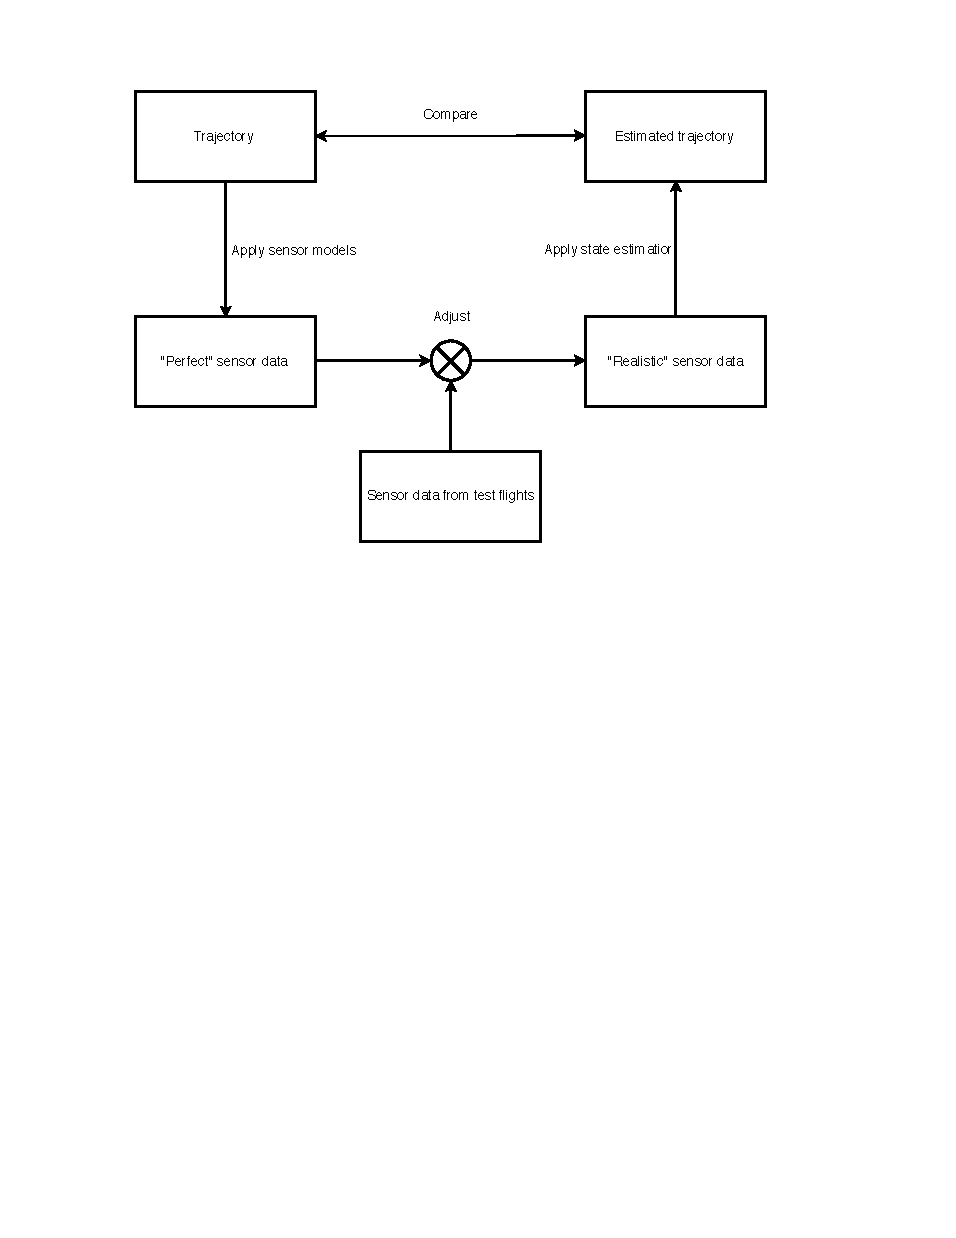
\includegraphics[width = \textwidth]{../BDADoku/Pictures/Verification.pdf}
   \caption{Verification Concept}
   \label{fig:Verification}
  \end{figure}

  \newpage
  The verification concept is based on a trajectory that is generated by a simulation, which should resemble a real trajectory as good as possible.
  This functionality was provided by the simulation team of ARIS from the last year's competition.
  The trajectory generated is then applied on the sensor models which are discussed below.
  The outcome is so called ``perfect'' sensor data which would represent the data provided by the sensor if they do not have any noise at all and the surroundings do perform as described.
  After that, noise is applied on this perfect sensor data which results in ``realistic'' sensor data. The inclusion of this noise will be discussed later in this chapter too. Basically this noise is drawn out of the sensor log data from the previous test flights.
  This ``realistic'' sensor data is then fed to the input of the different estimation algorithms which will provide their trajectory estimation at the output.

  Finally, to verify the functionality of these algorithms the estimated trajectory is compared against the generated trajectory.


  \section{Sensor models}
  As stated above the trajectory will be generated by the simulation.
  This simulation includes just the information for the height, so the sensor models have to be adjusted to generate the different needed data.
  The models are defined in the following parts.

  \subsection{Accelerometer}
  Perfect measuring data from the accelerometer (a) is simply put just the two times deviated height (h) by time (dt).
  $$a_z = \frac{d^2h}{dt^2}$$
  This value equals to the straight upwards acceleration. To get the acceleration which would be provided taking into account the x- and y-axis,
  the pitch angle $\varphi$ has to be calculated into this generated data like this.
  $$a_{pitch} = \frac{a_z}{cos(\varphi)} $$

  \subsection{Gyrometer}
  For the gyrometer there does not really exist a model with which those measurements could be generated.
  Therefore it has to be generated free handedly by taking the gyrometer measurements from the testflights into account.
  It has also to be stated that only the pitch angle of the rocket which can be seen in figure \ref{fig:RocketPitchAngle} is of interest for this first sensor fusion implementation.
  Because of this, only the pitch angle will be generated with random values which drive towards a realistic value that was read out of the data from test flights.

  \begin{figure}[h!]
    \centering
    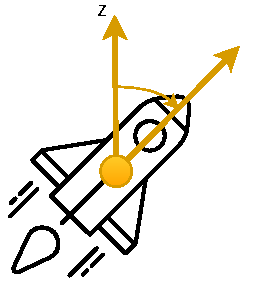
\includegraphics[width = 0.3\textwidth]{./Pictures/RocketSyMod.pdf}
    % RocketSyMod.pdf: 0x0 pixel, 300dpi, 0.00x0.00 cm, bb=
    \caption{Pitch angle visualisation}
    \label{fig:RocketPitchAngle}
  \end{figure}

  \newpage
  \subsection{Barometer}
  The barometer which are used in the aerospace usually provide the pressure in hP as well as the temperature in °C.
  \subsubsection{Pressure}
  To generated the pressure data the barometric height formula is used \cite{NASAEarthAtmosphereModel2015}.
  $$P = P0 \cdot (1- \frac{Tgrad\cdot h}{T0})^{\frac{M\cdot g}{R\cdot Tgrad}}$$
  \begin{tabbing}
  with: \= P0 = Pressure at ground level \\
  \> T0 = Temperature at ground level \\
  \> Tgrad = Temperature gradient for the actual weather condition \\
  \> M = Molar mass of Earth's air: 0.0289644 kg/mol\\
  \> g = Gravitational acceleration: 9.80665 m/$s^2$\\
  \> R = Universal gas constant: 8.3144598 J/mol/K\\
  \end{tabbing}

  This is more or less accurate until 11 000 meters above ground under the condition that the temperature gradient is determined correctly.

  \subsubsection{Temperature}
  Calculating the temperature out of the height is not trivial because the temperature gradient depends on the actual weather and the capacities of the air.
  So this gradient has to be determined before the start for each flight.

  $$T = T0 - Tgrad*h$$

  \subsection{GPS}
  The perfect GPS data is seen as the accurate height but with a slow sample rate around 0.5 to 2 Hz.
  This can simply be achieved by down sampling the height vector of the simulation with the right factor.

  \section{Noise Generation}
  To generate the different noises first the noise from the test flight has to be extracted.
  After this has been done, a system can be calculated which represents a white noise filter that generates noises
  that have the same spectral power density as the real noise. This process is visualised in figure \ref{fig:WhiteNoiseFilter}.

  \begin{figure}[h!]
 \centering
 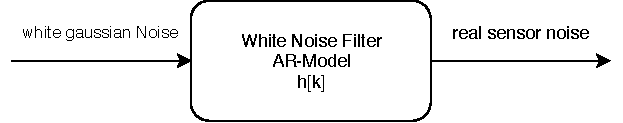
\includegraphics[width=0.5\textwidth]{./Pictures/WhiteNoiseFilter.pdf}
 % WhiteNoiseFilter.pdf: 0x0 pixel, 300dpi, 0.00x0.00 cm, bb=
 \caption{White noise filter concept}
 \label{fig:WhiteNoiseFilter}
\end{figure}


  For this the Yule Walker Equations should come in handy to calculate a so called auto regressive (AR) model of the noise system.
  An AR model is an all pole finite impulse response (FIR) system $a_1 \hdots a_N$ which generates a random sequence y[k] with a defined auto correlation value $\gamma_{yy}$ out of white gaussian noise $\omega[k]$.

  $$ y[k] = \omega[k] - \sum_{n=1}^{N} a_n \cdot y[k-n]  $$

  \newpage
  The Yule Walker Equations
  \begin{align*}
    \begin{bmatrix}
     \gamma_{yy}[0] & \gamma_{yy}[-1] & \dots & \gamma_{yy}[-N] \\
     \gamma_{yy}[1] & \gamma_{yy}[0] & \dots & \gamma_{yy}[-N+1] \\
     \vdots 		& \vdots 	& 	& \vdots	\\
     \gamma_{yy}[N] & \gamma_{yy}[N-1] & \dots & \gamma_{yy}[0]
    \end{bmatrix}
    & \cdot
    \begin{bmatrix}
     1 \\
     a_1 \\
     \vdots \\
     a_N
    \end{bmatrix}
    =
    \begin{bmatrix}
     \sigma^2_\omega \\
     0 \\
     \vdots \\
     0
    \end{bmatrix}
    \hfill
  \end{align*}
  \hfil \\
  estimate the coefficient $a_1 \dots a_N $ of the FIR system and the variance of the noise $\sigma^2_\omega $ which can be used to generate a random sequence which has the same auto correlation value $\gamma_{yy}$ and therefore the same spectral capacities as the input sequence y.
  Because the AR model consists of an all pole filter the noise should have a steady mean value. Preferably it should be zero mean for the estimated AR model to best represent the real system.
  For this the mean value of the measurements should be calculated beforehand and then be subtracted from them to get zero mean noises.
  After the generation of the desired noise this mean value can be readded again to represent the real sensors as good as possible.

  \section{System Model}
  The system model to represent the rocket will be hold simple to reduce the system load as well as to prevent non linearities.
  The most important values to estimate are the vertical height and speed, so
  for a first implementation just variables that determine those both will be used.
  This values are mainly calculated from the height provided by the GPS, the vertical acceleration from the accelerometer
  as well as the pressure and temperature from the pressure sensors. In addition to that the pitch angle from the gyrometer is used to calculate the pure vertical acceleration.
  But even with these simplifications there are different possible system description which have to be taken into account
  to find the best suitable.

  \subsection{General State Space System}
  For this quick view we have a look at the general notation of a state space system. First there is the update function:
  $$ \dot{x} = A \cdot x + B \cdot u + G \cdot q$$
  The A matrix resembles how the system changes over time by itself where the B matrix describes how input u influences the system.
  In addition noise on the system can be described with the G matrix and the noise input q.

  The second equation is the output equation:
  $$ y = C^T \cdot x + D \cdot u + R $$
  Here the $C^T$ matrix describes how the state value from x affects the output while the D matrix describes how inputs directly affect the output.
  The D matrix is zero in most state space systems, because in reality there are not many systems where the output directly and immediately reacts to the input.
  The noise on the output (measurement accuracy) can be described with the R matrix.

  \subsection{Point Mass}
  The most simple possible model would be that the rocket is resembled by a simple point mass which flies perfectly vertical upwards.
  For this only three state variables would be necessary: the vertical acceleration, the vertical speed and the height.
  $$x = \begin{bmatrix}
  h_z\\
  v_z\\
  a_z
  \end{bmatrix} $$
  This would reduce the A matrix of the general state space system to a 3x3 matrix with only two 1's in it.
   Also the input matrix would be set to a zero matrix in this model because the input process
  (power from the motor and drag force from the surrounding air) would be difficult to describe in such a linear system.
  \begin{align*}
  A = \begin{bmatrix}
  1 & 0 & 0\\
  0 & 1 & 0\\
  0 & 0 & 0
  \end{bmatrix}
  & \hspace{1cm}
  B = \begin{bmatrix}
          0 \\
          0 \\
          0 \\
  \end{bmatrix}
  \end{align*}
  In addition the measurements which are taken from the sensor will be described as the system output (y vector).
  So if the pressure from for example two barometers is calculated into the height beforehand it would result in the following output matrices.
 \begin{align*}
 y = \begin{bmatrix}
	  h_{GPS}	\\
          h_{p1}	\\
          h_{p2}	\\
          a_z
     \end{bmatrix}
    & \hspace{1cm}
 C^T = \begin{bmatrix}
         1 & 0 & 0	\\
	 1 & 0 & 0	\\
         1 & 0 & 0	\\
         0 & 0 & 1
        \end{bmatrix}
  \end{align*}

  As usual in engineering such a simplification comes with a cost. With this system description the output from the barometer would have
  to be transformed into the height before they could be taken into the system.
  Due to this the properties of these sensors could not be estimated correctly, because the value was transformed in a non-linear way before it entered the system.
  The same problem occurs with the accelerometer. If the rocket develops a pitch angle not equal to 0 while asccending, it would be measured wrong.
  To counter this error, the measurements of the accelerometer would have to be weighted by the angle of the gyrometer before entering the system.
  This weighting is also non-linear and the values of the gyrometer would not be filtered, which will make the estimation even more uncertain.

  \subsection{Point Mass with Pressure}
  To take into account the problems described above, the pressure can be taken into the state vector and therefore be estimated.
  $$ x = \begin{bmatrix}
  h_z\\
  v_z\\
  a_z\\
  p\\
  \end{bmatrix} $$
  While this solves the problems stated above it also produces a new. The system model can only describe linear dependencies between the state variables,
  but the relation between the pressure and the height is clearly non-linear in each atmospheric model.
  This dependency can be linearized, but if done so it does resemble the atmospheric model with less accuracy.
  Based on such a linearisation the barometer measurements can be interpolated so the actual pressure is available at any loop iteration.
  This results in a 4x4 A matrix and also an all zero B vector for the dynamics equation which look like this:
  \begin{align*}
  A = \begin{bmatrix}
         1    & 0 & 0 & 0    \\
         0    & 1 & 0 & 0    \\
         0    & 0 & 0 & 0    \\
         0    & KP_v & 0 & 0\\
        \end{bmatrix}
        & \hspace{1cm}
    B = \begin{bmatrix}
       0 \\
       0 \\
       0 \\
       0
      \end{bmatrix}
  \end{align*}

  This would also reflect on the output matrices which will directly contain the pressure.
  In addition the height calculated from the pressure can be inserted as an additional measurement to include them into the estimation.

  \begin{align*}
   y = \begin{bmatrix}
        h_{GPS}	\\
        h_{p}	\\
        a	\\
        p_1	\\
        p_2
       \end{bmatrix}
       & \hspace{1cm}
  C^T = \begin{bmatrix}
       1 & 0 & 0 & 0 \\
       1 & 0 & 0 & 0 \\
       0 & 0 & 1 & 0 \\
       0 & 0 & 0 & 1 \\
       0 & 0 & 0 & 1
      \end{bmatrix}
  \end{align*}
  The input matrix stays the same as above except of an additional dimension.

  \subsection{Point Mass with Angle and Pressure}
  The same solution as above can also be applied for the pitch angle.
  But its linearization and dependencies are more complicated and can therefore not be directly put into the system equation.
  This would change the state vector from above into the following.
  $$ x = \begin{bmatrix}
  h_z\\
  v_z\\
  a_z\\
  p\\
  \varphi_{pitch}\\
  \end{bmatrix} $$
  In consequence the dynamic part for A is extended into a 5x5 matrix while the B matrix still would be a zero vector.
  \begin{align*}
  A= \begin{bmatrix}
        0 & 1 & 0 & 0 & 0 \\
        0 & 0 & 1 & 0 & 0 \\
        0 & 0 & 0 & 0 & 0 \\
        0 & Kp_h & 0 & 0 & 0 \\
        0 & 0 & 0 & 0 & 0 \\
        \end{bmatrix}
  & \hspace{1cm}
  B = \begin{bmatrix}
             0 \\
             0 \\
             0 \\
             0 \\
             0 \\
        \end{bmatrix}
  \end{align*}

  In addition the output matrix and the y vector will also change to adjust for the gyrometer measurements.
  \begin{align*}
   y = \begin{bmatrix}
        h_{GPS} \\
        h_p \\
        a \\
        p_1\\
        p_2\\
        \varphi_{pitch}
       \end{bmatrix}
       & \hspace{1cm}
       C^T = \begin{bmatrix}
        1 & 0 & 0 & 0 & 0 \\
        1 & 0 & 0 & 0 & 0 \\
        0 & 0 & 1 & 0 & 0 \\
        0 & 0 & 0 & 1 & 0 \\
        0 & 0 & 0 & 1 & 0 \\
        0 & 0 & 0 & 0 & 1 \\
        \end{bmatrix}
  \end{align*}
  With this the pitch angle would be some sort of a real time low pass filter.
  This solution takes into account all measurements available for the needed values.
  It also keeps the calculation in the system as simple and linear as possible.

  \subsection{Discretisation}
  The systems stated above are all in continuous time state space description.
  To implement them on a discrete time system like a micro controller they have to be discretised.
  Those discrete matrices will be denoted with an additional lowercase d (A -> Ad).
  The general state space discrete description with noise looks as follows.
  $$ x[k+1] = Ad\cdot x[k] + Bd\cdot u[k] + Gd\cdot Q[k] $$
  $$ y = C \cdot x[k] + D\cdot u[k] + R[k] $$
  As can be seen, only the A, B and G matrices have to be discretised because
  the matrices used in the second equation are only there for scalar adjustment of the output
  and should therefore not contain any time depending calculation.
  The Ad matrix can be calculated with the the following formula.
  $$ Ad = e^{A\cdot Ts}$$
  Where Ts stands for the sampling time of the system which would be 1 millisecond on the system developed for this thesis.
  In addition there are two well known ways to calculate the other needed discrete matrices Bd and Gd.
  \begin{itemize}
   \item $$ Bd = Ad \cdot B $$
	 The first one resembles a perfect sampling which is equal to a multiplication with a dirac impulse (the value is measured in an infinitely small instant).
	 This calculation is rather far away from the reality because no sensor can measure with perfect dirac impluses.
	 The great advantage of this method on the other hand is its simple calculation.
   \item $$ Bd = \int_0^{Ts} e^{A\cdot v}\cdot B \ dv $$
	 This version does resemble a zero order hold as it is done by most sensors, so it is more realistic than the first version.
	 It comes at the cost that the calculation is more difficult \cite{DavidWSchultz2004}.
  \end{itemize}
  They can also be used in the same way to calculate Gd by changing B into G and Bd into Gd.
  Both version have to be tested in the simulation to see if the additional effort for the second version pays off enough.

  \section{State Estimator}
  There are several possibilities to generate the required sensor fusion. First of all an all new algorithm could be developed which accesses the
  stated problems directly. While this solution would be preferable regarding the probable high precision and efficency, the
  time and knowledge needed for this task would exceed the resources given for this thesis by far.
  Also as stated in chapter \ref{ch:Introduction} a lot of theoretical as well as practical pre-work has already been
  done and therefore should be used.
  So in the following different possible approaches with their pros and cons will be discussed.

  \subsection{Kalman Filter}
  First of all the traditional discrete Kalman filter has to be discussed as it provides the base for most known state estimators.
  Its structure provides the optimal estimation of the standard deviation estimation error as long as the noises are Gaussian
  and the observed system can be described by linear differential equations.
  But exactly there lies the problem: a physical system is seldom linear.
  Also the estimated system as well as its variances over the time have to be known to provide an optimal estimation.
  If the noise matrices of the system are static, the filter's gain matrices aim for a fix value and can therefore be calculated in beforehand.
  This reduces the computational effort by a significant amount \cite{DavidWSchultz2004}.
  It should be mentioned that even if the noise is not Gaussian the Kalman filter is still the best
  linear estimator as long as the system and its properties are well known \cite{SimonDan2006Ose:}.
  To summarise it, the discrete Kalman filter is a simple to understand and adjust state estimator in comparison to the following.

  \subsection{ROSE}
  The ROSE(rapid ongoing stochastic estimator) is put in simple terms three Kalman filters in one.
  Where the main filter is used as a normal Kalman filter as stated above, the additional two are used to estimated the
  the system noise as well as the measuring noise. Therefore this sensor preforms better than the traditional Kalman filter
  if those noises change over time in a not known fashion and has therefore also to be estimated.
  But higher accuracy comes to a cost, this sensor needs more computational effort to perform this estimations,
  because of the three Kalman filter equations which have to be calculated each step\cite{DavidWSchultz2004}.

  \subsection{Extended Kalman Filter}
  The extended Kalman filter provides additional parts to better access non linearities in the observed system.
  This by not estimating the state of the system but by estimating the linearised change of the state
  to the next coming state. For this the systems equations have to be derived around the current nominal point in every estimation state.
  This is some sort of bootstraping solution because the nominal points on which the derivation happens are estimated in the process and
  these estimates are then used to estimate the change between this estimation and the next.
  Therefore the computational effort needed raises even further because each function has to be deviated at each loop iteration \cite{SimonDan2006Ose:}.

  \subsection{Unscented Kalman Filter}
  The unscented Kalman filter uses the unscented transformation to calculate the different interpolating steps.
  The unscented transformation uses a test set of points around the current state and calculates the new values for them using the functions which represent the system.
  Out of these new values calculated from the test set the new state is estimated by weighting those new values depending on their probability of occuring.
  Using this approach the state function does not have to be linearized and therefore the estimation is most of the time better than that of the extended Kalman filter.
  But to achieve this the unscented Kalman filter needs to apply the unscented transformation onto the state vectors in each iteration. 
  As explained for this it calculates the estimation for many different values
  and does therefore need even more computational effort \cite{SimonDan2006Ose:}.

  \subsection{H$\infty$ Filter}
  The H$\infty$ filter is a more diverse approach than the ones described above.
  It was developed if the observed system and especially its noise is not well known.
  Put into other words it was developed to resemble an as robust as possible state estimator.
  In addition its stability can be easier guaranteed than that of a Kalman filter.
  But because he consists of additional tuning parameters to achieve this, he is more complicated to use than a Kalman filer.
  On the plus side the H$\infty$ filter minimises the worst-case estimation error in terms of the standard deviation of the estimation error compared to a Kalman filter \cite{SimonDan2006Ose:}.

  \newpage
  \section{Choosing}
  By taking the requirements table \ref{tab:Requirements} into the consideration for finding
  the optimal solution, two main requirements define this decision.
  The first one is the system load which is a critical requirement and has therefore to be achieved.
  The second one to specially take into account here is the modularity, so the algorithm should be as simple as possible.
  Taken into account that the system is more or less well known and that the noise can be
  determined with the simulation and the log data from previous test flights,
  a normal Kalman filter seems to be the most fitting solution.
  A more complicated approach should be avoidable, because the performance of the rocket and the sensor should stay the same during
  each flight.
  Because of this decision only the normal Kalman filter well be discussed from here on to fit the time limitations given for this thesis.
  Nonetheless the developed simulation should provide the possibility to implement and test the other state estimators in a later instalment.

  \subsection{Functionality}
  Since the best fitting state estimator has now been chosen, its detailed functionality shall be described here.
  This algorithm works in four main equations which can be divided into prediction and correction steps, as depicted in Figure \ref{fig:Kalmanfilter}.

  \begin{figure}[h!]
    \centering
    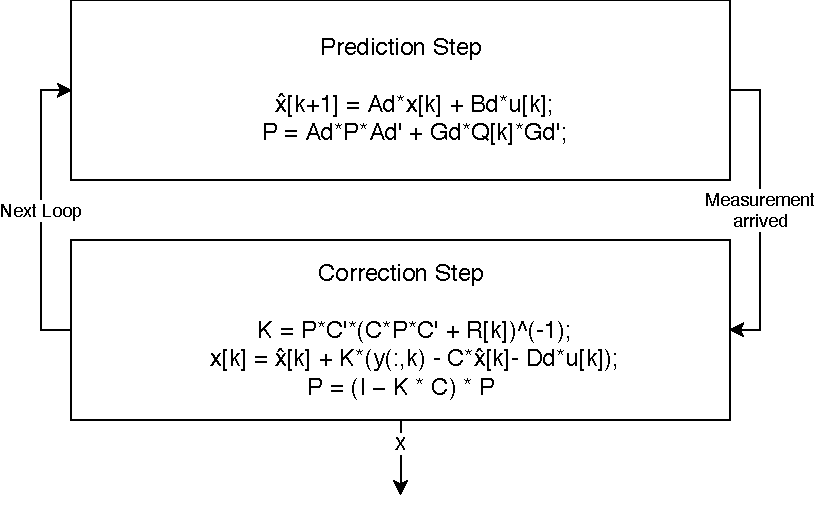
\includegraphics[width = \textwidth]{../BDADoku/Pictures/KalFIlFunc.pdf}
    \caption{Kalmanfilter}
    \label{fig:Kalmanfilter}
  \end{figure}

  \subsubsection{Prediction Step}
  The prediction equations take the current values of the state vector ($x[k]$)
  and uses the time depending system model part (Ad) to predict the state values for the next time step $\hat{x}[k+1]$ with the equation:
  $$ \hat{x}[k+1] = Ad\cdot x[k] + Bd\cdot u[k] $$
  The hat denotes that this value is an assumption.

  In addition the certainty matrix (P) is estimated with the same tactic, which means that it is calculated how trustworthy those predictions are.
  $$ P = Ad\cdot P\cdot Ad^T + Gd\cdot Q[k]\cdot Gd^T$$
  For this the system noise is used, so with the help of the Q matrix it can be stated how well known the system is in this
  time step.

  \subsubsection{Correction Step}
  If the measurements arrive those will be used in the correction step to correct the prediction.
  First the Kalman gain (K) is calculated with the equation.
  $$ K = P\cdot C^T\cdot (C \cdot P \cdot C^T + R[k])^{(-1)} $$
  This uses the P matrix from the prediction step as well as the R matrix which represents the noise on the measurements, meaning how accurate the values from the measurements are.
  K is then used in the following equation to calculate $x[k]$:
  $$x[k] = \hat{x}[k] + K\cdot (y[k] - C\cdot \hat{x}[k]-Dd\cdot u[k])$$
  By this, the measurement corrects the predicted value of the state vector with there uncertainties taken into account \cite{DavidWSchultz2004}.

  In the last equation $$P = (I − K * C) * P $$ the certainty matrix is corrected with the help of the Kalman gain and the estimated certainty matrices.

  To be able to run this Kalman filter the matrices for the system models (Ad,Bd,C,D), the measurements noise (Q,Gd) as well as the system noises (R) have to be defined.



